\documentclass[pdftex, 12pt, a4paper]{article}

\usepackage[pdftex]{graphicx}
\usepackage[utf8x]{inputenc}
\usepackage{appendix}
\usepackage{cite}
%\usepackage{pgfgantt}
%\usepackage{pst-gantt}
\usepackage{rotating}
\usepackage{pdflscape}
\usepackage{hyperref}
%\usepackage{breakurl}
\usepackage{listings}
\usepackage{nomencl}
\usepackage[a4paper]{geometry}
\usepackage{tabularx}
\usepackage{longtable}

\nomitemsep 1pt

\makenomenclature

\begin{document}

\begin{titlepage}

\begin{center}

{\large Electronics and Computer Science\\
Faculty of Physical and Applied Sciences\\
University of Southampton}\\[5em]

{\large A Group Design Project report submitted for the award of MEng
Computer Science}\\[5em]

{\large Thomas Grainger}\\
{\large Weike Liao}\\
{\large Chris Orchard}\\
{\large Nafiseh Vahabi}\\[5em]

{\large Project Supervisor: Tim Chown\\
Second Examiner: Les Carr}\\[5em]

{\LARGE A Trending Topic Malware Crawler}\\[5em]
{\large \today}\\[5em]


\end{center}

\end{titlepage}


\begin{abstract}
The project sets out to determine if those who distribute malicious content
use trending topics on services such as Twitter or the News Media so as to
gain some of the traffic from users searching for legitimate information about
those topics.

The project discusses design and implementation of a distributed framework
designed to organise multiple subsystems that process trending topics from
these sources and emulate a user browsing for pages related to those trending
topics. In the process those pages accessed are evaluated for malicious
content hoping to distribute malware to unsuspecting users using drive by
download toolkits.

\end{abstract}

\tableofcontents
%acknowledgments
\section*{Acknowlegements}
\addcontentsline{toc}{section}{Acknowledgments}

Our customer Team Cymru and their representative Chas Tomlin.

The Celery community, in particular Ask Solem Hoel (@asksol) 

Proof Reading: Ali Emamy, Matthew Power, Chrissie Metcalf
%project description (problems + goals)
\section{Introduction}

%chris's intro stuff
\subsection{Emma Watson and Malware}
On September 10th 2012, MacAfee released a report detailing a list of the top 20
celebrities that it believed were the most risky to search for on the internet\cite{mac-watson}.
The report specifies a number of threats from risky web sites, such as malware,
phishing, and spam, and determined that Emma Watson was the most risky celebrity
to search for on the web with more than 12.6\% chance of a site being malicious
when searching for her name combined with phrases such as ``free download''.

The hypothesis suggested in the MacAfee report is that trending topics have
malicious web pages crafted specifically to target the topic, and this is the
hypothesis that will be investigated in the project.

Before investigating if malware is targeted at trending topics, it is necessary to
invstigate exactly what constitutes a trending toic. ``Trending topic'' is a term
that originates from Twitter, where statistics are collected on users tweeting
with a given hashtag and used to determine popular hashtags, presented in the
user interface a ``trending topic''. When discussing trending topics in this
report, other sources of trends and popular subjects will also be considered as
trending topics.

To make it possible to invesitgate the hypothesis proposed above a framework
will be designed and build to automatically gather trends, search for URLs
relating to the trends, and then attempt to detect whether the URL is hosting
malicious content. The data will then be collected into a database, allowing the
hypothesis to be tested. Results will be reported using a web interface that
will also be capable of monitoring the status of the malware scanning system.

%nafiseh's intro stuff
\section{Introduction}

\subsection{Problem Definition}

The continually increasing variety of known and unknown malwares make malware detection a difficult problem to solve. As malware detection systems become more intelligent and sophisticated, malware writers are also developing more advanced methods. Some anti-virus software is ineffective in terms of detecting unknown malware. This project seeks to design a malware detection system capable of identifying web pages containing malicious content for a given contextual topic as represented by trending search keywords. 
Also, this research involved emulating a user browsing for these keywords. The challenging part of this project arose in seeking to define a malicious web page, as there are many variations of an infected webpage depending on the type of malware. 
Some types of malware directs the user to an illegal website by clicking on the URL. A large group of malware are designed with a commercial objective in mind. A webpage that has poor content, offers no goods or services and is used for the purpose of directing users to unsolicited advertisements is an example of commercial malware. Whilst other web pages may look perfectly fine at first glance but in fact contain malicious functions, for example by using JavaScript functions. In the case of the latter, the detection is even more difficult because the malware is a type of obfuscation malware that is hidden from the user. Moreover, malwares could come from a variety of different sources.
The examples above highlight the difficulties of this project. Furthermore, whilst a great deal of research has been performed on the subject of malware detection and the effectiveness of various detection methods, such research specifically considered a specifically defined type of malware and analysed the methods used for that particular malware. 
In seeking to propose a malware detection system capable of identifying web pages containing malicious content based on trending search keywords, this paper gives consideration to the fact that different variations of malware exist. 


%literature review 
\section{Literature Review}

Previous reports in the relevant areas were researched. In this section we are
going to introduce some background knowledges and research contributions
summarised from three reports written by authoritative institutions. We will
see the importance of trending keywords in malware distribution, and the
methods and systems to measure and counter them. Approaches for malicious
website detection and analysis are also included. 

\subsection{Search-engine optimization} 

Search engine is a key tool for
exploring resources on the Internet and becomes increasingly significant in
people's daily life. Many famous search engines index web pages are using PageRank
algorithm, which states that the rank of a web page depends on the quantity and
quality of incoming links, and the higher is the rank, the more likely that the
web page will apear in the top results of a search query. Although search
engine providers do not usually reveal their algorithms in calculating
PageRanks in order to reduce spammers who gaming with the system, many main
features are still well-known. For example, many webpages have their main title
stored in the URLs, therefore the URLs themself may represent a summary of the
page contents, which is a feature that can be utilised by website administrators 
to rise PageRank.
\paragraph{}
A report produced by University of Washington and Microsoft
Research Silicon Vally introduces a widely used search results poisoning
technique named Search Engine Optimization (SEO) as well as a system that
automatically detects them, called deSEO.\cite{deseo} They claim to be "the
first to present a systematic study of search-result poisoning attacks and how
to detect them". SEO is a process that uses varies approaches to affect a web
page such that it will apear in higher positions of a search engine's search
results, and for most of the cases, a rise of PageRank is achieved. This
process can be exploited to support illegal websites, such as malicious
websites, with some additional unethical techniques (which will be introduced
later) therefore achieves conspicuous boosts in PageRanks. This is called SEO
attacks. According to the paper, a typical SEO attack consists three servers,
which are compromised server, redirection server and exploit server. The
process of exploitation can be divided into five steps: 
\paragraph{}
\begin{enumerate} 
\item The victim submit a common request to a search engine.
\item The victim click on a search result and is navigated to a malicious web
page hosted on a compromised server.
\item The compromised server fowards the request to a redirection server.
\item The redirect server selects an exploit server then navigates the user
to it.  
\item Exploitation of the vitim's browser or scareware displayed.  
\end{enumerate}

To compromise a server, the attackers often target specific popular software
with known vunlerabilities but are still used by many servers. The example in
the report is a shopping websites management software called osCommerce, and
the attackers compromise the servers by uploading php scripts. Those scripts
are likely to have funtions that can navigate through the server's file system,
find data, and upload further files etc. When a server is compromised, SEO
pages can then be generated. Those pages contains a large number of links
connects to other SEO pages (probably on other compromised servers), as well as
contents that relate to the keywords this page's URL focuses on. Such dense
link structure and high relevant contents are the main means to elevate the
PageRank. The generated SEO pages may have clocking techniques, which means
they present different contents to search engine crawlers and victims. When the
page is visited by a search engine crawler, links to other SEO pages and
poisoned keywords are displayed, and when a victim accesses, the user's browser
is forwarded to a redirection server. 

\paragraph{}
Redirection servers are often formed
with several layers before reaching the exploit server, where they redirect
within the compromised server network. In the paper's case the domains of those
servers are very similar and according to their IPs it is determined that those
servers are hosted in physical groups. The Exploit servers in that example have
191 domains being hosted on only two IPs, and the webpage is very cautious with
incoming visitors. The page detects search engine crawlers as well as referrer,
and also blocks IPs from search engine companies.  

\paragraph{} 
The
researchers of the report crawled across the network of SEO links and finially
determined 5400 compromised domains. Each domain have an average links of
80,000 to other domains with 8,000 keywords corresponding to the same number of
SEO pages, which proves the use of dense link structure in rising PageRank.
They also provided an estimation of the number of victims affected by this
group of domains, which was produced from a dataset collected for two and a
half months. The result was that over 81,000 users were directed to exploit
pages.
\paragraph{} 
The detection of SEO attacks is not a trivial task, as
those pages usually trigger malicious actions only after strict requirements
are met, such as depending on the execution result of a JavaScript with the
input of a user's mouse action. Fortunately the report proved that study only
the URLs' structures is sufficient to complete the detections. 


\subsection{Trending-term exploitation}
Beside from how a SEO attack is technically implemented, we wonder what kind 
of websites apply SEO and how those SEO pages are found by victims. SEO is a 
process of improving PageRank, and before a webpage's PageRank is taken into 
account their content must match with the keywords of a search query. Many
well-known public websites and search engines provide trending data in real
time (such as Google Trends and Twitter Trends), and the easiest method to
determine what people are searching is to collect trending keywords/terms. With
trending terms the webpage's contents are then usually generated by sending
search queries with those terms, and combine contents in the URLs returned.
\paragraph{}
In this section we focus on a report researching ad-filled and malicious
websites.\cite{fashioncrime} It claims to be the "first large-scale measurement
and analysis of trending-term exploitation on the web", and as a result they
concluded the ways of trending terms application in spams among the web, with a
huge dataset collected through nine months containing over 60 million search
results. The report includes a wide research from trending terms collection to 
economics analysis, however here we only introduce topics relevant to our 
project. 
\subsubsection{Data collection and classification}
A trending terms dataset is categorised into trending set and control set. 
Trending set is formed by fast-changing popular terms, obtained from Google 
Hot Trends. These terms will become "cooled" in near future and are dropped 
from the dataset if so. Control set consists constantly popular search 
keywords, with the purpose to find out any "phenomena unique to the trending 
nature". The terms are then automatically fed to search-engines with optimised 
time interval. According to their experiments, 85\% of results are identical 
when comparing the results obtained from tests with 10 minutes and 4 hours 
interval, and finially 4 hours interval is applied to all their programs. Top 
results of each search query are stored in the dataset for classification, 
where in their case 32 results of Google and 100 results of Yahoo! are used.
\paragraph{}
In the report they organise websites into three categories, benign, 
malware-distributing and ad-filled, where ad-filled sites are also called Made 
for AdSense (MFA). For malware-distributing sites they simply check them with 
Google Safe Browsing API, in contrast for MFA sites they developed a 
supervised machine-learning algorithm then completed it with 363 manally 
inspected MFA sites as training set. As a result, for all URLs collected, 
0.30\% from the trending set and 0.13\% from the control set are determined to 
have malware and 6.2\% from the trending set are MFA sites. 
\subsubsection*{Measurement of trending-term abuse}
This report referred number of times to John et al.\cite{deseo}, which we 
reviewed in previous section. The authors confirmed dense link structures in 
both MFA and malware-serving websites. For MFA sites they built a directed 
graph and proved the existence of a "fairly large, collusive MFA operation" 
who owns 30.7\% of all MFA sites, and for malware-serving websites, as 
reported in the previous section, they found that a large portion of 
compromised servers are controlled by a single group, named a campaign. The 
same pattern appears in Twitter posts containing MFA links. Their data 
illustrates that 50\% of the MFA tweets direct to only 7.2\% of MFA domains 
across all MFA domains involved in Twitter. 
\paragraph{}
The authors then carried out a research in examining characteristics of 
trending terms. They classify trending keywords with Google Insights for 
Search, then find out the peak popularity estimate and advertising value 
provided by Traffic Estimator for each keyword. An observation is that all 
categories of keywords are targeted by malware and MFA, however the 
distribution of malicious sites varies according to a keyword's popularity and 
advertising value. More specifically, referring to their data, the percentages 
of malware-distribution and MFA sites decrease as the keyword's peak 
popularity and advertising value rises. They also conclude that, as a source 
of revenue, "malware and MFA behave more like substitutes, rather than 
complements".  
\subsubsection{Search-engine intervention}
Google stated some modifications of its search-engine ranking algorithm in 
response of increasing SEO behaviors on 24th Februrary, 2011. As the date was 
between their project's data collection duration, the report includes an 
investigation of the effectiveness about this announcement. \\
They compared the percentage of MFA sites in top 10 search results, with the 
conclusion states a decrease from 3.1\% to 0.47\% after a month later to the 
announcement date. They also collected the number of visits to MFA sites, 
which proved that the visits to MFA sites using Google ads had been decreased 
by 41\%, where those without had a reduction of 93\%. 

\subsection{Automatic malware collection}
We have introduced one of the most popular means to distribute malware (SEO) 
with trending terms as a significant role. In this section we will know the 
methods to detect malicious websites and analysis malwares in them, and 
finially collects malicious code across the web. A report carried out by Korea 
Internect \& Security Agency\cite{automalwarecollecting} explained a system 
that collects malicious code from malware-distributing websites found by 
search-engine with trending keywords. The report presents three approaches 
categorised into active and passive for detecting whether a website is 
malicious: 
\begin{enumerate}
\item 
{\bf Passive Malware Detection}\\
In this method we let attackers infest the system, then perform local analysis 
with the malware. Server honeypot is an example of this approach, which hosts 
a vunlerable system and waits for exploitation.   
\item
{\bf Active Low Interaction Client Honeypot}\\
In this case the malicious website is accessed, with only HTML downloaded 
however not executed. Static analysis is then applied to the file. The main 
advantage of this approach is simplicity. This kind of honeypots requires 
minimal resources to maintain and employ and does not give visible 
risks.\cite{honeypots}
However limitation exists. The most obvious point is this kind of systems are 
designed to detect known threats, because there is no way to find out the 
behaviors of a new type of attack without executing them. Another problem is 
that we are unable to check the contents of a page if it contains interative 
scripts which cannot be downloaded. For example, a block of script may require 
sources from other files, which we cannot examine further without running it. 
\item
{\bf Active High Interaction Client Honeypot}\\
The term high interaction means the malicious webpage is actually visited by a 
real browser under a real vunlerable system. 
The file system and registory are then scanned for modification. This approach 
requires a light-weight operating system which can be reset without 
significant time cost. An obvious advantage is that a thorough test can be 
performed to avoid any dynamic content cannot be found by static analysis, 
which means we are able to collect further amount of information includes the 
full behavior of an attack. Another point is that the high interaction system 
does not predict how the attack will behave, instead it gives an open 
environment which monitors all activities.\cite{honeypots}
However it is still not perfect, as some malicious code may require specific 
enviroment in order to execute, such as a certain version of browser and 
operation system combination. The system also requires significantly more 
resources than low interaction methods, including memory, disk space and 
computing power. 
\end{enumerate} 
The two active methods can be combined to overcome their shortages, which 
creates a new hybrid method. 
\paragraph{}
In the report they implemented an automated malware collecting system 
ultilises both low and high interaction approaches. The overall execution flow 
of their system is as follwing:
\begin{enumerate}
\item Trending keywords (or ``search keyword that reflects the social issue'' 
as the report said) are collected from various search engines. Though details 
in this step is not described in the report. 
\item Search queries are sent with those trending terms to a number of search 
engines. The top URLs returned are stored in a URL dataset. 
\item A URL component check is performed as a low interaction detecting 
method. For each URL they download and crawl the webpage to find out any 
suspecious behaviours. The checked criteria including the existence of zero 
size iFrame, the intensity of obfucated scripts, frequency of \% symbol and 
frequncy of particular function calls. They discovered that an 
obfuscated JavaScript in a malicious webpage usually contains significantly 
longer unique character streams, and similar patterns occur for \% symbol 
frequency and function calls. In the end they concluded a term called web page 
entropy which sums all the features described above, which can be used to 
classify whether a webpage is malicious or not. 
\item Webpages recongnized as malicious are sent to a high interaction client 
honeypot which automatically visits the page and collects malicious code 
distributed. They utilise a single virtual machine with the most vulnerable 
environment, however details about the environment are not included. They 
isolate newly created files and prevent their execution while also normalise 
any obfuscated scripts downloaded. 
\end{enumerate} 
\paragraph{}
In the performance verification section a comparison of 
their system and other existing active malware detection systems (HoneyMonkey, 
HoneyClient and MonkeySpider) shows that the new hybrid one has significant 
advantages in static analysis, false positive rate and system recovery speed. 
It is also the only system that is able to recover obfuscated script and 
pre-process URLs. 
\paragraph{}
Their data collection period spans for one and a half month, resulting 1287 
unique suspecious file collected. They test these files in two steps: first 
scan them with commercial anti-virus software, four vaccine programs were used 
in their case,  then for the remaining non-virus files they send them to 
behavior analysis systems such as ThreatExport and Norman SandBox. As a result 
a total of 986 are determined to be malicious, where 119 of them are only 
discovered by behavior analysis systems. 
The URLs are collected from search-engines, email spams and blacklists. 
Unfortunately the report does not include details about the source and 
quantity of their trending terms, and size of the URL dataset is also unknown. 

\section{Related work}

Over the past few years, the internet has been used by an attacker to distribute a malware. Search engines can be used as a medium for spreading a malware through the internet. Essentially, attackers use the search engine optimisation algorithm applied by Google to insert their malicious links in the most visited websites. Based on deSEO observations, attackers used trendy keywords and regenerated relevant content pages in order to achieve a successful attack\cite{deSEO}.

Therefore, a recent study has been undertaken to detect the malicious links based on such trendy keywords. In this study, the proposed detection method identifies suspicious websites by analysing the components of the URLs. In the second step, each suspicious websites is clustered based upon its lexical structures. Finally, a cluster analysis is undertaken in order to select the suspicious group\cite{deSEO}.
The dataset required for this experiment was collected from Google and Bing search engines. The data set was divided into two groups, the first group was used for training and the second group was used for the purpose of learning. The system can automatically identify additional malicious URLs. However, detection will most probably fail if the attacker does not use the keyword in the URL\cite{deSEO}.

A recent study undertaken in 2011, analyzed the increasing amount of malware that related to the trendy-terms. This research provides the first large-scale measurements of using trending terms in web search engines over a period of nine months. This research how the attackers use trending keywords to direct users to advertising websites. These websites profit by displaying advertisements on their webpage without offering any goods or services\cite{moore2011fashion}.
The proposed methodology is based on data collection and website classification. The data for this study is collected from different sources such as Google, Bing and Twitter. The websites are classified into two groups, malicious and benign. The malicious websites can be a malware hosting website, or may contain advertisements\cite{moore2011fashion}.

According to this paper, their system added hot trendy topics to the list of trendy term every hour and removed older terms from the list after 14 days. The result of their measurements showed that a high percentage of the malware belonged to Google Hot trending topics. Also, the comparison between trendy terms and popular topics highlighted that both topics were valuable tools for attackers in distributing the malware. However, trendy terms returned a higher number of infected webpages. The difference being that a popular topic can last for a longer period of time and its related website always has visitors, whilst a trendy term will stay popular as a ‘hot topic’ for a short period of time and have a lot of visitors during that short time period\cite{moore2011fashion}.
%Specification + Customer Feedback (--> Design)
\section{Specification}
To aid in the task of designing the solution, a set of requirements have been drawn up. These requirements have been derived from the division of the task presented in the goals of the project with MOSCOW priority attached to each.

\begin{enumerate}
    \setlength{\itemsep}{1pt}
    \item The system \textbf{must} be able to collect trends
    \item The system \textbf{should} be able to collect trends from more than once source
    
    \item The system \textbf{must} be able to discover target web pages using a search engine
    \item The system \textbf{should} be able to discover target web pages using multiple different search engines
    \item The system \textbf{could} be able to discover target web pages using Twitter
    
    \item The system \textbf{must} be able to determine if a page is malicious or not
    \item The system \textbf{must} be able to control multiple different malware scanning components
    \item The system \textbf{must} use High Interaction malware Scanning
    \item The system \textbf{must} use Zero Interaction malware Scanning
    \item The system \textbf{must} use Low Interaction malware Scanning
    \item The system \textbf{should} be able to dispatch dispatch only likely candidate malicious URLs to slower High Interaction Scanners
    \item The system \textbf{should} be able to fine tune High Interaction Scanner dispatch probability
    \item The system \textbf{could} use historical speed and current status of the system to influence High Interaction Scanner dispatch probability

    \item The system \textbf{must} be able to store data determined about targets
    \item The system \textbf{must} be able to relate data about targets to the trend source and time it was discovered on
    \item The system \textbf{must} be able to generate reports
    \item The system \textbf{should} be able to show the time taken for a particular 
    \item The system \textbf{could} display reports dynamically using a web based interface
    \item The system \textbf{should} be able to monitor the status of the system
    \item The system \textbf{should} be able to monitor the status of each malware scanning component
    \item The system \textbf{could} be able to display statuses with a web interface
\end{enumerate}

\section{Customer Interaction}
The project was put forward by Team Cymru Research NFP, ``a specialized Internet security research firm and 501(c)3 non-profit''\cite{team-cymru}. Team Cymru maintains various real-time monitoring ``pods'' to measure the status of malware on the public Internet. The project compliments their existing offerings by incorporating social media and news trends with active web scanning.

Over the course of the project the group had two meetings with Team Cymru representative Chas Tomlin: a video conference and an informal meeting.  Meetings were intended to occur at the start of the project and after each of the presentations, however only one of the post-presentation meetings occurred.

The video conference was used to introduce the group to Team Cymru and discuss the project requirements, in which the brief was expanded upon. The specification was influenced by requests to:
\begin{enumerate}
    \item A requirement to emulate a user browsing the web using a virtualized web browser also referred to as High Interaction Malware Scanning.

    \item A requirement to use simple crawling and static analysis as in Low Interaction Malware Scanners, to be determined as part of the literature search.

    \item A suggestion to create a scanning modules that uses signature oriented scanning of pages and the hyper-linked files

    \item A suggestion to write modules that make use of existing repositories of malicious websites such as Google's Safe Browsing API\cite{google-safe} Google's Safe Browsing API and the crowd sourced Web Of Trust.

    \item Make the code machine-independant, so as to allow the scanning modules to operate on cheap, commodity, cloud machines such as Amazon Web Services Spot Instances\cite{aws-spot} or Rackspace Cloud instances\cite{rackspace}
\end{enumerate}

Also discussed was the possibility of downloading and investigating a ``Drive by Download'' malicious software distribution tool.  The legal considerations of downloading and executing an illegal piece of software are complex and as such would require the group to obtain a detailed set of permissions before attempting such a task.

While researching this as a possibility because of such considerations it was determined that the time and effort required to obtain permissions to would be prohibitive the decision was made to not investigate ``Drive By Download'' toolkits as part of the project.

After the first presentation an informal meeting was held to discuss progress on the project so far with Chas:

\begin{enumerate}
    \item A suggestion to use Internet Explorer 6 running under several interfaces of Wine to act as a faster High Interaction malware scanner than virtualizing an entire operating system.

    \item A suggestion to use ClamAV as the scanning engine behind the signature oriented scanning malware scanner.

    \item Lowered the requirement of a web based reporting interface from \textbf{should} to \textbf{could}, as being able to manually query the database would be acceptable.

    \item A requirement to be able to monitor the system, components and workers specifically mentioning Nagios, however it was chosen to use Celery's own monitoring tools instead
\end{enumerate}

One further meeting was to be held after the second presentation, but Chas was not available.

\nomenclature{API}{Application programming interface}

%Group work approach
\section{Planning \& Group-Work Approach}

\subsection{Development of a Plan}


\subsection{Group-work Approach}

\subsection{Risk Managment}

\subsection{Stakeholder Management}

Writing Brief
Developing a Plan
Division of Work (skills based)
Progression of Work
Customer/Stakeholder Management
PM Approach, Risks
Development Approach (Agile)


%justified design
\section{Architectural Design}
\section{High interaction malware detection with Wine}
\subsection{Design}
In this section we discuss one of our high interaction malware detection 
approach in details. High interaction requires completely functionable systems 
and realistic user interaction with the target malicious websites, which means 
it will certainly consume more system resources and demands more complicated 
framework compared to low interation and no interaction methods. The major 
feature of this approach is the capability of detecting unknown malicious 
actions. In this project we developed our own system called Wine Explorer 
which complys this approach. It uses Wine as a compatibility layer to run 
Internet Explorer 6 in our Linux environment and is capable to scan for 
possible file operations performed by malicious websites. 

\subsubsection{Wine Is Not an Emulator}
Wine is a widely used free software which acts as a compatibility layer 
capable of running Windows applications on non-Windows operating 
systems.\cite{wikiwine} Not like virtual machines and emulators which simulate 
internal Windows logic, ``Wine translates Windows API calls into POSIX calls 
on-the-fly, eliminating the performance and memory penalties of other methods 
and allowing you to cleanly integrate Windows applications into your 
desktop.''\cite{aboutwine} Hence the acronym Wine stands for ``Wine Is Not an 
Emulator''. The fact is that Wine is able to run most Windows applications 
without any performance drop as long as there is no performance related bugs, 
especially for 2D applications. Although technically say, Wine requires an 
extra layer on the top of the system, there is no differences to programs that 
uses extra libraries. An exact example of such software is the compatibility 
mode in new versions of Windows for running legacy 
software.\cite{wineperformance} \\
Wine is definitely better than conventional virtual machines as well. Although 
virtual machines have advantages in simulating programs which give more 
realistic environments, they are certainly not resource saving. In most of the 
case, a virtual machine consumes significantly more memory, disk space and 
CPU, as it needs to simulate the whole operating system instead of a single 
program like Wine does. Wine treats Windows applications as first-class 
citizens, which run at full speed.\cite{wineperformance} \\
Wine uses a working directory as a complete Windows system which stores all 
information about the specific system's configurations and files in its virtual 
hard drive. Moreover, the active working directory is known as the Wine prefix. 
One of our discoveries about Wine is that the creation of Wine prefix is 
lightweight and resource saving compared to that of a virtual machine or
emulator, while the Wine prefix itself also conforms to the nature of a 
sandbox, which means all kind of behaviours performed by programms inside the 
Wine prefix cannot affect the underlying system. Therefore we conclude that 
Wine is a suitable tool to create a client honeypot in high interaction 
malware detection. \\

\subsubsection{Execution Flow}
Wine Explorer is a straightforward program, and the following graph 
illustrates the execution flow of detecting a single URL. \\
% Flow chart here
With Wine Explorer we open the URLs given by the URL classifier introduced 
previously with the specific instance of Internet Explorer inside the Wine 
prefix. 
Those URLs are said to be strongly suspecious of containing malware and are 
supposed to be investigated in depth. 
In order to speed up Wine prefix creation, we pack a clean Wine prefix with 
Internet Explorer 6 installed. Therefore whenever a new Wine prefix is needed, 
we just unpack it to a desired location. 
The package's SHA-256 hash is calculated and stored in Wine Explorer such that 
its validity can be ensured. 
The package is then uploaded into a web drive and can be downloaded in 
order to increase the system's portability. \\
The system should also be able to store multiple instances of Wine prefixes 
and execute Internet Explorers in them concurrently. 
After an execution is completed a scan is performed to check file system 
modifications inside that Wine prefix. 
Due to various reasons the file system might have changes performed by normal 
operations such as cache files. 
Therefore at this step we provide a white list which describes the kind of 
files that should be ignored, which is applied to filter the results. 
The results are then returned to the main system and the Wine prefixes after 
scanning should be removed in order to save disk space. 

\subsection{Implementation}
We use Python to implement this program just as other parts of our project. 
In the program an instance of Wine prefix running Internet Explorer is called 
a WineBrowser, which is a threaded class manages all operations with a single 
given URL. This is how the program work in details:
\begin{enumerate}
\item
Check cache for the package containing the predefined Wine prefix, if not 
exist download it, then perform a hash check.
If success the package is unpacked to a temporary directory. 
In the file system there should also be a clean Wine prefix unpacked from the 
package, which is used for checking file system changes later. 
\item
The active Wine prefix is set to the temporary directory, and the Internet 
Explorer is run with the given URL under Wine. 
\item
Wait for 30 seconds.
\item
Check the file system changes. This is achieved by running filecmp recursively 
for all files between the clean Wine prefix and the active one. The results 
are filtered against a white list then returned to the main system. The white 
list is included in the appendix TODO. 
\item
The temporary directory is removed. 
\end{enumerate}
We choose 30 seconds as the waiting interval is because of possible network 
latency. Any webpages take more than 30 seconds to load will be discarded 
as if not they will significantly lower the system's throughput. \\
The main system runs WineBrowser instances with Celery, one per task, in order 
to achieve concurrent execution of multiple Wine programs at the same time, 
which increases the overall throughput dramatically. 
\subsection{Testing}
After the first draft of implementation of the Wine Explorer, its functions are
tested individually before combine to a whole module for unit testing. This is a sample 
output from \verb'check_change' when comparing a modified Wine prefix with 
the clean one:
\begin{verbatim}
(['wineprefix_ie6', 'user.reg~'], 
['winetricks.log'], 
['user.reg'], 
[])
\end{verbatim}
Each array in the record stores newly created files, removed files, 
modified files and files the system is unable to check respectively. 
\paragraph{}
In conclusion, all functions 
explained in the implementation section are ensured to work separately, 
however the websites that affect file systems are yet to be found. 
This program will be further polished when we produce a demo 
of the whole project in the future. 




\subsection{Evaluation}



\subsection{Design}
Trend Analysis Tasks should be implemented to take advantage of multiple different sources of trending topics to be used as keywords for URL Discovery tasks.

Sourced that should be used are Twitter Trending Topics API, RSS Feeds and trends from derived from the Sun JSON Feed.

It is important to note that further possibilities for keyword determination should be researched. The sources suggested here are the ones easiest to interface to, but might not be the sources malware distribution networks actually use.

\subsubsection{Twitter}
The twitter api is available in multiple versions, 1 and 1.1. Currently 1 is deprecated and it is recommended that new applications build against 1.1.  The disadvantage of the 1.1 API is that it requires a ``User Context'', ie all requests must be authenticated based on Application-User key.

The Twitter API provides access to global trending topics at

\verb`https://api.twitter.com/1.1/trends/place.json`

Documented at \verb`https://dev.twitter.com/docs/api/1.1/get/trends/place`

The keyword information is available at [0].trends[].name.

Topics with a \# in-front are Twitter ``hashtags'', and are usually camel cased. The system should be able to convert from camel cased to space delimited. As in \url{http://commons.apache.org/lang/api-3.0.1/org/apache/commons/lang3/StringUtils.html#splitByCharacterTypeCamelCase%28java.lang.String%29}.

Eg. \#BrazilWantsOneDirection -> Brazil Wants One Direction
\#XFactorPHFinale -> X Factor PH Final

In the case of all capitals eg NIALLSAYHITOTURKEY an entirely lowercase keyword should be derived.

\subsubsection{RSS}
A set of RSS feeds should be collected and parsed, ``feedparser'' is likely to be useful for this.

Each item from a feed should be entered into a corpus, to calculate keywords from items in the corpus algorithms such as TFIDF should be used. The natural language library ``metanl'' is likely to be helpful.

Note that each feed can be processed separately. Ie one corpus per feed.

\subsubsection{The Sun JSON API}
The Sun provides a JSON API for the top 200 most commented on articles at \verb`http://bootstrap.thesun.fyre.co/api/cust/ni/todays_hottest/200.json`. In most cases the content of this JSON file can be treated exactly the same as an RSS feed however care should be taken to deal with the dodgy encoding of some of the returned headlines: ``Terry a â\\u0080\\u0098liarâu\\0080\\u0099'' should be ``Terry a \"liar\"''.

\subsubsection{Alternative Sources}
Examples include:
\begin{itemize}
    \item Link aggregation sites such as Reddit and Digg.
    \item Search engine common searches and trends such as Google, Bing and Yahoo trends services.
    \item Network logs such as the campus search trends. It should be noted that this data is very unlikely to be accessible by malware distribution networks and might allow us to see trends before they do.
\end{itemize}

%implementation
\subsection{Implementation}
The most popular Twitter library for Python is called Tweepy, which is also 
our choice. This library provides access to Twitter version 1.1 API, which 
requires OAuth authentication. Therefore we created a Twitter account 
dedicated for this program, which provides consumer key and access token in 
order to pass the authentication. \\
The program then retrieves global trending keywords from the Twitter's {\em 
trends/place} API. As previous described, in order to cope with keywords with 
hashtags, we implemented a hashtag handler, who's role is to remove the hash 
tag and convert the camel case word to sentence case. This is achieved by 
applying regular expression substitution: \\
\newline
\verb`re.sub(r'((?<=[a-z])[A-Z]|(?<!\A)[A-Z](?=[a-z]))',r' \1',camelCaseString)`
\newline
Before the conversion happens the keyword is also decoded into unicode. The 
reason is that Celery does not support Python 2 strings which may lead to 
crash when Celery is sending them to RabbitMQ. 
\paragraph{}
We also hard coded a list of famous news websites' RSS feed addresses in the 
program, the website list includes BBC, NewYork Times, Guardian, The Washington 
Post and so on. Our RSS parser downloads every feeds, parses them into list 
then extracts news titles in them. Characters require encodings other than 
UTF-8 are ignored. The downloading is achieved with requests and any network 
errors will be handled gracefully. 
\paragraph{}
The top 200 commented articles from Sun JSON API are handled in a similar way 
as that of RSS feeds. Due to good compatibility between Python and JSON we 
were able to extract article titles without any difficulties. 
\paragraph{}
Twitter trends, RSS feeds and Sun JSON are implemented as three different 
functions which are going to be run as separate Celery tasks. All of them 
return a list of keywords or sentences to the main system. 

\paragraph{URL Discovery}
The URL discovery phase is called with a keyword from the Trend Analysis phase and should query a search engine to determine a set of pages related to those URLs. This phase is designed to emulate a user searching for pages.

To determine URLs to investigate a search engine of some sort is required, the best I have found that can be used by automata is http://dogpile.co.uk.

\paragraph{Dogpile}

A handy code snippet for retrieving URLs from dogpile:

map(lambda link: link.get('href'),lxml.html.fromstring(requests.get("http://www.dogpile.co.uk/search/web?q=foo").text).cssselect(".webResult .resultDisplayUrl"))

Because each of the links we want is wrapped in a ``ClickHandler'' \verb`http://cs.infospace.com/ClickHandler.ashx?du=http%3a%2f%2fwww.ietf.org%2frfc%2frfc3092.txt&ru=http%3a%2f%2fwww.ietf.org%2frfc%2frfc3092.txt&ld=20121006&ap=10&app=1&c=uk.dogpl&s=dogpileuk&coi=239138&cop=main-title&euip=94.193.128.47&npp=10&p=0&pp=0&pvaid=1351848139fc4226b6b6a0f6e0eed58b&ep=8&mid=9&hash=22AE450C7F5B9FA7C51FE2CEA7841093`

The URLs returned must be parsed, eg using ``urlparse'' to retrieve the unwrapped URL available in the ``du'' or ``ru'' GET parameter, in this case\cite{rfc3092}

%BEGIN INCLUDED TECH SECTIONS HERE
\section{Malware Lists}
\section{High interaction malware detection with Wine}
\subsection{Design}
In this section we discuss one of our high interaction malware detection 
approach in details. High interaction requires completely functionable systems 
and realistic user interaction with the target malicious websites, which means 
it will certainly consume more system resources and demands more complicated 
framework compared to low interation and no interaction methods. The major 
feature of this approach is the capability of detecting unknown malicious 
actions. In this project we developed our own system called Wine Explorer 
which complys this approach. It uses Wine as a compatibility layer to run 
Internet Explorer 6 in our Linux environment and is capable to scan for 
possible file operations performed by malicious websites. 

\subsubsection{Wine Is Not an Emulator}
Wine is a widely used free software which acts as a compatibility layer 
capable of running Windows applications on non-Windows operating 
systems.\cite{wikiwine} Not like virtual machines and emulators which simulate 
internal Windows logic, ``Wine translates Windows API calls into POSIX calls 
on-the-fly, eliminating the performance and memory penalties of other methods 
and allowing you to cleanly integrate Windows applications into your 
desktop.''\cite{aboutwine} Hence the acronym Wine stands for ``Wine Is Not an 
Emulator''. The fact is that Wine is able to run most Windows applications 
without any performance drop as long as there is no performance related bugs, 
especially for 2D applications. Although technically say, Wine requires an 
extra layer on the top of the system, there is no differences to programs that 
uses extra libraries. An exact example of such software is the compatibility 
mode in new versions of Windows for running legacy 
software.\cite{wineperformance} \\
Wine is definitely better than conventional virtual machines as well. Although 
virtual machines have advantages in simulating programs which give more 
realistic environments, they are certainly not resource saving. In most of the 
case, a virtual machine consumes significantly more memory, disk space and 
CPU, as it needs to simulate the whole operating system instead of a single 
program like Wine does. Wine treats Windows applications as first-class 
citizens, which run at full speed.\cite{wineperformance} \\
Wine uses a working directory as a complete Windows system which stores all 
information about the specific system's configurations and files in its virtual 
hard drive. Moreover, the active working directory is known as the Wine prefix. 
One of our discoveries about Wine is that the creation of Wine prefix is 
lightweight and resource saving compared to that of a virtual machine or
emulator, while the Wine prefix itself also conforms to the nature of a 
sandbox, which means all kind of behaviours performed by programms inside the 
Wine prefix cannot affect the underlying system. Therefore we conclude that 
Wine is a suitable tool to create a client honeypot in high interaction 
malware detection. \\

\subsubsection{Execution Flow}
Wine Explorer is a straightforward program, and the following graph 
illustrates the execution flow of detecting a single URL. \\
% Flow chart here
With Wine Explorer we open the URLs given by the URL classifier introduced 
previously with the specific instance of Internet Explorer inside the Wine 
prefix. 
Those URLs are said to be strongly suspecious of containing malware and are 
supposed to be investigated in depth. 
In order to speed up Wine prefix creation, we pack a clean Wine prefix with 
Internet Explorer 6 installed. Therefore whenever a new Wine prefix is needed, 
we just unpack it to a desired location. 
The package's SHA-256 hash is calculated and stored in Wine Explorer such that 
its validity can be ensured. 
The package is then uploaded into a web drive and can be downloaded in 
order to increase the system's portability. \\
The system should also be able to store multiple instances of Wine prefixes 
and execute Internet Explorers in them concurrently. 
After an execution is completed a scan is performed to check file system 
modifications inside that Wine prefix. 
Due to various reasons the file system might have changes performed by normal 
operations such as cache files. 
Therefore at this step we provide a white list which describes the kind of 
files that should be ignored, which is applied to filter the results. 
The results are then returned to the main system and the Wine prefixes after 
scanning should be removed in order to save disk space. 

\subsection{Implementation}
We use Python to implement this program just as other parts of our project. 
In the program an instance of Wine prefix running Internet Explorer is called 
a WineBrowser, which is a threaded class manages all operations with a single 
given URL. This is how the program work in details:
\begin{enumerate}
\item
Check cache for the package containing the predefined Wine prefix, if not 
exist download it, then perform a hash check.
If success the package is unpacked to a temporary directory. 
In the file system there should also be a clean Wine prefix unpacked from the 
package, which is used for checking file system changes later. 
\item
The active Wine prefix is set to the temporary directory, and the Internet 
Explorer is run with the given URL under Wine. 
\item
Wait for 30 seconds.
\item
Check the file system changes. This is achieved by running filecmp recursively 
for all files between the clean Wine prefix and the active one. The results 
are filtered against a white list then returned to the main system. The white 
list is included in the appendix TODO. 
\item
The temporary directory is removed. 
\end{enumerate}
We choose 30 seconds as the waiting interval is because of possible network 
latency. Any webpages take more than 30 seconds to load will be discarded 
as if not they will significantly lower the system's throughput. \\
The main system runs WineBrowser instances with Celery, one per task, in order 
to achieve concurrent execution of multiple Wine programs at the same time, 
which increases the overall throughput dramatically. 
\subsection{Testing}
After the first draft of implementation of the Wine Explorer, its functions are
tested individually before combine to a whole module for unit testing. This is a sample 
output from \verb'check_change' when comparing a modified Wine prefix with 
the clean one:
\begin{verbatim}
(['wineprefix_ie6', 'user.reg~'], 
['winetricks.log'], 
['user.reg'], 
[])
\end{verbatim}
Each array in the record stores newly created files, removed files, 
modified files and files the system is unable to check respectively. 
\paragraph{}
In conclusion, all functions 
explained in the implementation section are ensured to work separately, 
however the websites that affect file systems are yet to be found. 
This program will be further polished when we produce a demo 
of the whole project in the future. 




\subsection{Evaluation}




\section{Clam AV}
\section{High interaction malware detection with Wine}
\subsection{Design}
In this section we discuss one of our high interaction malware detection 
approach in details. High interaction requires completely functionable systems 
and realistic user interaction with the target malicious websites, which means 
it will certainly consume more system resources and demands more complicated 
framework compared to low interation and no interaction methods. The major 
feature of this approach is the capability of detecting unknown malicious 
actions. In this project we developed our own system called Wine Explorer 
which complys this approach. It uses Wine as a compatibility layer to run 
Internet Explorer 6 in our Linux environment and is capable to scan for 
possible file operations performed by malicious websites. 

\subsubsection{Wine Is Not an Emulator}
Wine is a widely used free software which acts as a compatibility layer 
capable of running Windows applications on non-Windows operating 
systems.\cite{wikiwine} Not like virtual machines and emulators which simulate 
internal Windows logic, ``Wine translates Windows API calls into POSIX calls 
on-the-fly, eliminating the performance and memory penalties of other methods 
and allowing you to cleanly integrate Windows applications into your 
desktop.''\cite{aboutwine} Hence the acronym Wine stands for ``Wine Is Not an 
Emulator''. The fact is that Wine is able to run most Windows applications 
without any performance drop as long as there is no performance related bugs, 
especially for 2D applications. Although technically say, Wine requires an 
extra layer on the top of the system, there is no differences to programs that 
uses extra libraries. An exact example of such software is the compatibility 
mode in new versions of Windows for running legacy 
software.\cite{wineperformance} \\
Wine is definitely better than conventional virtual machines as well. Although 
virtual machines have advantages in simulating programs which give more 
realistic environments, they are certainly not resource saving. In most of the 
case, a virtual machine consumes significantly more memory, disk space and 
CPU, as it needs to simulate the whole operating system instead of a single 
program like Wine does. Wine treats Windows applications as first-class 
citizens, which run at full speed.\cite{wineperformance} \\
Wine uses a working directory as a complete Windows system which stores all 
information about the specific system's configurations and files in its virtual 
hard drive. Moreover, the active working directory is known as the Wine prefix. 
One of our discoveries about Wine is that the creation of Wine prefix is 
lightweight and resource saving compared to that of a virtual machine or
emulator, while the Wine prefix itself also conforms to the nature of a 
sandbox, which means all kind of behaviours performed by programms inside the 
Wine prefix cannot affect the underlying system. Therefore we conclude that 
Wine is a suitable tool to create a client honeypot in high interaction 
malware detection. \\

\subsubsection{Execution Flow}
Wine Explorer is a straightforward program, and the following graph 
illustrates the execution flow of detecting a single URL. \\
% Flow chart here
With Wine Explorer we open the URLs given by the URL classifier introduced 
previously with the specific instance of Internet Explorer inside the Wine 
prefix. 
Those URLs are said to be strongly suspecious of containing malware and are 
supposed to be investigated in depth. 
In order to speed up Wine prefix creation, we pack a clean Wine prefix with 
Internet Explorer 6 installed. Therefore whenever a new Wine prefix is needed, 
we just unpack it to a desired location. 
The package's SHA-256 hash is calculated and stored in Wine Explorer such that 
its validity can be ensured. 
The package is then uploaded into a web drive and can be downloaded in 
order to increase the system's portability. \\
The system should also be able to store multiple instances of Wine prefixes 
and execute Internet Explorers in them concurrently. 
After an execution is completed a scan is performed to check file system 
modifications inside that Wine prefix. 
Due to various reasons the file system might have changes performed by normal 
operations such as cache files. 
Therefore at this step we provide a white list which describes the kind of 
files that should be ignored, which is applied to filter the results. 
The results are then returned to the main system and the Wine prefixes after 
scanning should be removed in order to save disk space. 

\subsection{Implementation}
We use Python to implement this program just as other parts of our project. 
In the program an instance of Wine prefix running Internet Explorer is called 
a WineBrowser, which is a threaded class manages all operations with a single 
given URL. This is how the program work in details:
\begin{enumerate}
\item
Check cache for the package containing the predefined Wine prefix, if not 
exist download it, then perform a hash check.
If success the package is unpacked to a temporary directory. 
In the file system there should also be a clean Wine prefix unpacked from the 
package, which is used for checking file system changes later. 
\item
The active Wine prefix is set to the temporary directory, and the Internet 
Explorer is run with the given URL under Wine. 
\item
Wait for 30 seconds.
\item
Check the file system changes. This is achieved by running filecmp recursively 
for all files between the clean Wine prefix and the active one. The results 
are filtered against a white list then returned to the main system. The white 
list is included in the appendix TODO. 
\item
The temporary directory is removed. 
\end{enumerate}
We choose 30 seconds as the waiting interval is because of possible network 
latency. Any webpages take more than 30 seconds to load will be discarded 
as if not they will significantly lower the system's throughput. \\
The main system runs WineBrowser instances with Celery, one per task, in order 
to achieve concurrent execution of multiple Wine programs at the same time, 
which increases the overall throughput dramatically. 
\subsection{Testing}
After the first draft of implementation of the Wine Explorer, its functions are
tested individually before combine to a whole module for unit testing. This is a sample 
output from \verb'check_change' when comparing a modified Wine prefix with 
the clean one:
\begin{verbatim}
(['wineprefix_ie6', 'user.reg~'], 
['winetricks.log'], 
['user.reg'], 
[])
\end{verbatim}
Each array in the record stores newly created files, removed files, 
modified files and files the system is unable to check respectively. 
\paragraph{}
In conclusion, all functions 
explained in the implementation section are ensured to work separately, 
however the websites that affect file systems are yet to be found. 
This program will be further polished when we produce a demo 
of the whole project in the future. 




\subsection{Evaluation}




\section{Capture-HPC}
\section{High interaction malware detection with Wine}
\subsection{Design}
In this section we discuss one of our high interaction malware detection 
approach in details. High interaction requires completely functionable systems 
and realistic user interaction with the target malicious websites, which means 
it will certainly consume more system resources and demands more complicated 
framework compared to low interation and no interaction methods. The major 
feature of this approach is the capability of detecting unknown malicious 
actions. In this project we developed our own system called Wine Explorer 
which complys this approach. It uses Wine as a compatibility layer to run 
Internet Explorer 6 in our Linux environment and is capable to scan for 
possible file operations performed by malicious websites. 

\subsubsection{Wine Is Not an Emulator}
Wine is a widely used free software which acts as a compatibility layer 
capable of running Windows applications on non-Windows operating 
systems.\cite{wikiwine} Not like virtual machines and emulators which simulate 
internal Windows logic, ``Wine translates Windows API calls into POSIX calls 
on-the-fly, eliminating the performance and memory penalties of other methods 
and allowing you to cleanly integrate Windows applications into your 
desktop.''\cite{aboutwine} Hence the acronym Wine stands for ``Wine Is Not an 
Emulator''. The fact is that Wine is able to run most Windows applications 
without any performance drop as long as there is no performance related bugs, 
especially for 2D applications. Although technically say, Wine requires an 
extra layer on the top of the system, there is no differences to programs that 
uses extra libraries. An exact example of such software is the compatibility 
mode in new versions of Windows for running legacy 
software.\cite{wineperformance} \\
Wine is definitely better than conventional virtual machines as well. Although 
virtual machines have advantages in simulating programs which give more 
realistic environments, they are certainly not resource saving. In most of the 
case, a virtual machine consumes significantly more memory, disk space and 
CPU, as it needs to simulate the whole operating system instead of a single 
program like Wine does. Wine treats Windows applications as first-class 
citizens, which run at full speed.\cite{wineperformance} \\
Wine uses a working directory as a complete Windows system which stores all 
information about the specific system's configurations and files in its virtual 
hard drive. Moreover, the active working directory is known as the Wine prefix. 
One of our discoveries about Wine is that the creation of Wine prefix is 
lightweight and resource saving compared to that of a virtual machine or
emulator, while the Wine prefix itself also conforms to the nature of a 
sandbox, which means all kind of behaviours performed by programms inside the 
Wine prefix cannot affect the underlying system. Therefore we conclude that 
Wine is a suitable tool to create a client honeypot in high interaction 
malware detection. \\

\subsubsection{Execution Flow}
Wine Explorer is a straightforward program, and the following graph 
illustrates the execution flow of detecting a single URL. \\
% Flow chart here
With Wine Explorer we open the URLs given by the URL classifier introduced 
previously with the specific instance of Internet Explorer inside the Wine 
prefix. 
Those URLs are said to be strongly suspecious of containing malware and are 
supposed to be investigated in depth. 
In order to speed up Wine prefix creation, we pack a clean Wine prefix with 
Internet Explorer 6 installed. Therefore whenever a new Wine prefix is needed, 
we just unpack it to a desired location. 
The package's SHA-256 hash is calculated and stored in Wine Explorer such that 
its validity can be ensured. 
The package is then uploaded into a web drive and can be downloaded in 
order to increase the system's portability. \\
The system should also be able to store multiple instances of Wine prefixes 
and execute Internet Explorers in them concurrently. 
After an execution is completed a scan is performed to check file system 
modifications inside that Wine prefix. 
Due to various reasons the file system might have changes performed by normal 
operations such as cache files. 
Therefore at this step we provide a white list which describes the kind of 
files that should be ignored, which is applied to filter the results. 
The results are then returned to the main system and the Wine prefixes after 
scanning should be removed in order to save disk space. 

\subsection{Implementation}
We use Python to implement this program just as other parts of our project. 
In the program an instance of Wine prefix running Internet Explorer is called 
a WineBrowser, which is a threaded class manages all operations with a single 
given URL. This is how the program work in details:
\begin{enumerate}
\item
Check cache for the package containing the predefined Wine prefix, if not 
exist download it, then perform a hash check.
If success the package is unpacked to a temporary directory. 
In the file system there should also be a clean Wine prefix unpacked from the 
package, which is used for checking file system changes later. 
\item
The active Wine prefix is set to the temporary directory, and the Internet 
Explorer is run with the given URL under Wine. 
\item
Wait for 30 seconds.
\item
Check the file system changes. This is achieved by running filecmp recursively 
for all files between the clean Wine prefix and the active one. The results 
are filtered against a white list then returned to the main system. The white 
list is included in the appendix TODO. 
\item
The temporary directory is removed. 
\end{enumerate}
We choose 30 seconds as the waiting interval is because of possible network 
latency. Any webpages take more than 30 seconds to load will be discarded 
as if not they will significantly lower the system's throughput. \\
The main system runs WineBrowser instances with Celery, one per task, in order 
to achieve concurrent execution of multiple Wine programs at the same time, 
which increases the overall throughput dramatically. 
\subsection{Testing}
After the first draft of implementation of the Wine Explorer, its functions are
tested individually before combine to a whole module for unit testing. This is a sample 
output from \verb'check_change' when comparing a modified Wine prefix with 
the clean one:
\begin{verbatim}
(['wineprefix_ie6', 'user.reg~'], 
['winetricks.log'], 
['user.reg'], 
[])
\end{verbatim}
Each array in the record stores newly created files, removed files, 
modified files and files the system is unable to check respectively. 
\paragraph{}
In conclusion, all functions 
explained in the implementation section are ensured to work separately, 
however the websites that affect file systems are yet to be found. 
This program will be further polished when we produce a demo 
of the whole project in the future. 




\subsection{Evaluation}





%END INCLUDED TECH SECTIONS

\nomenclature{SSL}{Secure Sockets Layer}
\nomenclature{HTTP}{Hypertext Transfer Protocol}
\nomenclature{REST}{Representational state transfer architecture}

\subsubsection{Presentation of Data}



%\section{Classification}

\subsection{Implementation}

\subsubsection{URL Database}

An important part of the classification algorithm is the dataset used for the purpose of the clustering. The dataset in this project contains examples of both malicious and benign URLs. Diagram 2.1 illustrates the structure of the dataset.  

%Diagram 2.1 The Snapshot of Dataset in the classification.

The results from the five malware scanners along with the associated confidence rate is saved to the classification database. Therefore, after running the detection system, the database is updated and the new URLs are added to the database. For the purpose of pattern matching, the system developed included the capability of converting the contents of the database into the Python dictionary.

\subsubsection{Classification Unit}
 
The classification unit is where the data clustering is performed. Initially, the plan was to employ the machine learning methods in the classification algorithm. The most popular machine learning methods for clustering are; Naïve Base, Support Vector Machine (SVM) and Decision Tree. Employing the machine learning methods requires a predefine dataset for the purpose of training and learning data. Therefore, any unknown URL can be identified based on the learning data. According to the observation of the deSEO research and IMDS project, the results will be reliable and promising. [Ref: deSEO, IMDS]
However, despite the initial plan and advantage of using machine learning methods for the classification, it was not possible to apply such methods for this project for to the following reasons:
1-	The project is time limited  
2-	The result of malware scanner modules will not be available until the end of the project.

Therefore, an alternative approach was adopted for the classification unit. This relies on pattern matching between two URLs, one being the new URL and the other the database URLs. For pattern matching, each URL is deemed to be a string, so an algorithm is required to perform the matching between the two strings. A few string measurement algorithms were attempted with the most suitable being selected. A brief description of the attempted algorithms is as follows;

\paragraph{Fuzzy String Searching}
			
This is a technique used to search for the closest match for a given string. It is also called Approximate String matching. As its definition suggests, this technique does not produce an exact match for a given sequence. Furthermore, its implementation is complex and the algorithm is quite slow \cite{String-match}.

\paragraph{Sequence mining}

Sequence mining is a popular algorithm used in data mining. Data mining is a process to find a pattern in a dataset. This algorithm tries to find similar patterns between two sequences and is used in Bioinformatics and for predicting DNA sequences. Sequence mining algorithm is remarkably efficient, and this attribute makes the algorithm suitable for implementing in other applications. However, the algorithm is used for sequences that have a restricted number of alphabet characters. Therefore, given the variation of URLs in the dataset, this algorithm is not appropriate for this project\cite{Sequence-mining}  

\paragraph{Jaro–Winkler distance}

The Jaro-Winkler distance algorithm is popular in computer science and is also applied in statistics. This algorithm aims to find similarities between two strings by assigning a confidence rate ranging from zero to one to the result of the algorithm. If the result is zero, there is no similarity between two strings, whilst a result of one means there is an exact match for the two strings. This method gives an accurate result when comparing short strings such as a person’s name. However, for lengthy URLs, the application of this method produces a poor result. Therefore, this method is rejected for use in the implementation stage because the result would only be reliable for short URLs\cite{Jargo-winkle}. 

\paragraph{Levenshtien Distance}
	
Levenshtien distance is one of the strings metrics that measures the minimum number of edits required to convert one sequence to another. It is sometimes called edit distance. In this measurement the following edit operations are permitted; deletion and insertion. 
Formally, the Levenshtien distance is defined by the mathematic formula below;
Suppose x and y are two given strings, the Levenshtien distance between x and y are;
%insert mathematic formula
%
%\begin{equation}

%Lev_()= 

%\label{Levenshtien formula}
%\end{equation}
%
In the above definition, there are three cases corresponding to minimum. The first element is for deletion from x to y, the middle case is for insertion and the last element relates to whether x and y match or mismatch\cite{Levenshtein}.  

For example, the Levenshtien distance between “http://www.bbc.co.uk/news/world/” and “http://www.bbc.co.uk/news/wales/” involves four steps before the first URL is converted to the second, as shown below:

1-	(substitution of "a" for "o")
http://www.bbc.co.uk/news/world/ -> http://www.bbc.co.uk/news/warld/

2-	(deletion of “r”)
http://www.bbc.co.uk/news/warld/ -> http://www.bbc.co.uk/news/wald/

3-	(Insertion of “e” after “l”)
http://www.bbc.co.uk/news/wald/-> http://www.bbc.co.uk/news/wale/

4-	(Insertion of "s" at the end)
http://www.bbc.co.uk/news/wale/ -> http://www.bbc.co.uk/news/wales/

According to the Levenshtien distance, it is not possible to transform the first URL to the second one with fewer than four edits. The main advantage of using this method is that two URLs do not need to have same number of characters. Hence, a URL with any structure is acceptable as an input for the classification. However, adapting the Levenshtien distance for pattern matching can reduce the speed of the system.

After analysing different methods for pattern matching and considering their advantages and drawbacks, the Levenshtien distance was selected and implemented in the classification.  Therefore, when a new URL enters the system, the classification unit searches the database to find a match to the new URL. There are three possibilities as a result of this matching. Firstly the new URL may already exist in the system; in which case a result is immediately returned with a one hundred percent confidence rate. The latter result determines whether the new URL is malicious or benign. The second possible outcome of the classification unit is that a result is returned with a poor confidence rate. In this case the new URL will be sent to the heavyweight scanning module to undertake more scanning processes. Thirdly, a pattern matching result showing a high confidence rate would follow the lightweight scanning process.
The advantage of incorporating a classification module within the malware detection system is increased efficiency. More importantly, the system is capable of identifying unknown URLs, which many commercial virus scanners are not able to detect. 

\subsection{Testing}
After the first draft of implementation of the Wine Explorer, its functions are
tested individually before combine to a whole module for unit testing. This is a sample 
output from \verb'check_change' when comparing a modified Wine prefix with 
the clean one:
\begin{verbatim}
(['wineprefix_ie6', 'user.reg~'], 
['winetricks.log'], 
['user.reg'], 
[])
\end{verbatim}
Each array in the record stores newly created files, removed files, 
modified files and files the system is unable to check respectively. 
\paragraph{}
In conclusion, all functions 
explained in the implementation section are ensured to work separately, 
however the websites that affect file systems are yet to be found. 
This program will be further polished when we produce a demo 
of the whole project in the future. 




%Evaluation, Project Management Summary (gantt comparison etc.)
\subsection{Evaluation of Wine Explorer}
Wine Explorer is indeed a feasible approach for high interaction malware 
detection. As Wine is a compatibility layer instead of virtual machine or 
emulator, the Internet Explorers running under it can execute in full speed, 
where the computation resource consumption is minimal compared to what 
a virtual machine or emulator require. The applications run by Wine are also 
treated as ``first class citizens''\cite{wineperformance} such that 
permissions for them are not 
restricted. The creation of a Wine prefix is also impressively fast, which 
means the overhead for honeypot reset is minimal. \\
However disadvantages still exists. We explained that the Wine prefix is treated
as a sandbox, and the reason is almost all Windows applications do not operate 
with Linux environment. Imagine if attackers predicted the Wine Explorer 
environment, then they could easily develop Windows applications which inject 
Linux shell commands, which means, they will have access to the file system 
outside of Wine prefix. Also, the suspicious behaviour detection functions of 
this program is really naive which cannot cover all situations. An example 
could 
be a downloaded virus that is able to delete itself before the scan begins. 
During that time it is sufficient to perform illegal behaviours such as 
sensitive information collection. The modification of system 
registry is also not considered in this application. According to the project 
schedule we are unable to achieve everything perfectly due to the approaching 
deadline. 

\subsection{Project Management Summary}

\subsubsection{Time Management Record}

To effectively manage time over the course of the project the group constructed
a gannt chart to track the components tasks of the project and to fit those tasks into the
tight schedule defined by the project guidelines. To build the gantt chart the
group first plotted the milestones of the project (shown as diamonds on the
gantt chart); submitting a brief to the
customer, the two progress seminars, the report hand-in and the final
presentation. The time between the milestones formed the development cycles
used in the project, with two iterations of development of four weeks in length
each before each progress seminar. One week at the end of each iteration was
left for preparation of the progress seminar.

At the end of the first iteration, the group was on time with the deliverables
set in the plan, and there was time during the preparation of the first progress
seminar to integrate the code produced and present a demo of the framework
retrieving trends and URLs. After the progress seminar the group started work on
the malware scanners, having researched scanning methods during the first
iteration. When preparing for the second progress seminar, the group started to
suspect that the task of creating and integrating malware scanners into the
framework was harder than originally estimated, resulting in development effort
continuing after the second progress seminar in contrast to the plan. The
consequence of this was reduction in scope for the the amount of results
collected, and the delay of the web reporting interface to an additional task
completed after the delivery of the rest of the project but still in time for
presenting to the customer at the final presentation.

The Gantt charts can be found at the end of the project management summary.

\subsubsection{Writing the Report}

Although the first words of the report were written in early November, writing
the report started in earnest at the beginning of December. To aid the group
with assessing current progress with the report, a python script was written
that shows a day by day cumulative word count drawn on a stacked bar chart with
one segment per group member. The output of the python script is shown below.
This script uses the github API and texcount.pl script to count words in each
commit in the repository.

AWESOME REPORTIFICATE GRAPH

\subsubsection{Achievements \& Lessons Learnt}

The total length of time available to complete the project in was 11 weeks, in
this time the group had to fit in a customer brief, two presentations, and a
24000 word report. This meant that the effective development time for the
project was in the region of 4-6 weeks. In this time the group managed to
construct a working framework that could collect trends from a number of
sources, retrieve URLs related to those trends, and conduct rudimentary analysis
of the URLs for malware. As of writing the only working malware scanners are
those which involve the very lowest levels of interaction. Whilst the
Capture-HPC scanner was successfully integrated into the framework, further
configuration of the system is needed before it can be used to process URLs in
an effective way. The other malware scanners are not yet fully integrated into
the framework. Given the time constraints, the group managed to achieve most of
the work needed for a fully featured protoype and it is expected that it will be
possible to demo a completed version of the project at the final presentation to
the customer. In retrospect the scope of the project was very wide, and perhaps
a more complete product could have been delivered if the scope had been reduced
somewhat.

Another lession learned during the course of the project relates to the division
of work. The style of development was intended to allow a reasonable degree of
autonomy, but still provide ample opportunity for the group members to assit
each other with tasks in case of difficulty. An unintended consequence of this
was that no one group member had complete knowledge of all of the technical
aspects of the system, making integration more complicated and hence causing
delays.


\clearpage
\begin{landscape}
\subsection{Gantt Charts}
\begin{figure}[htb]
\centering
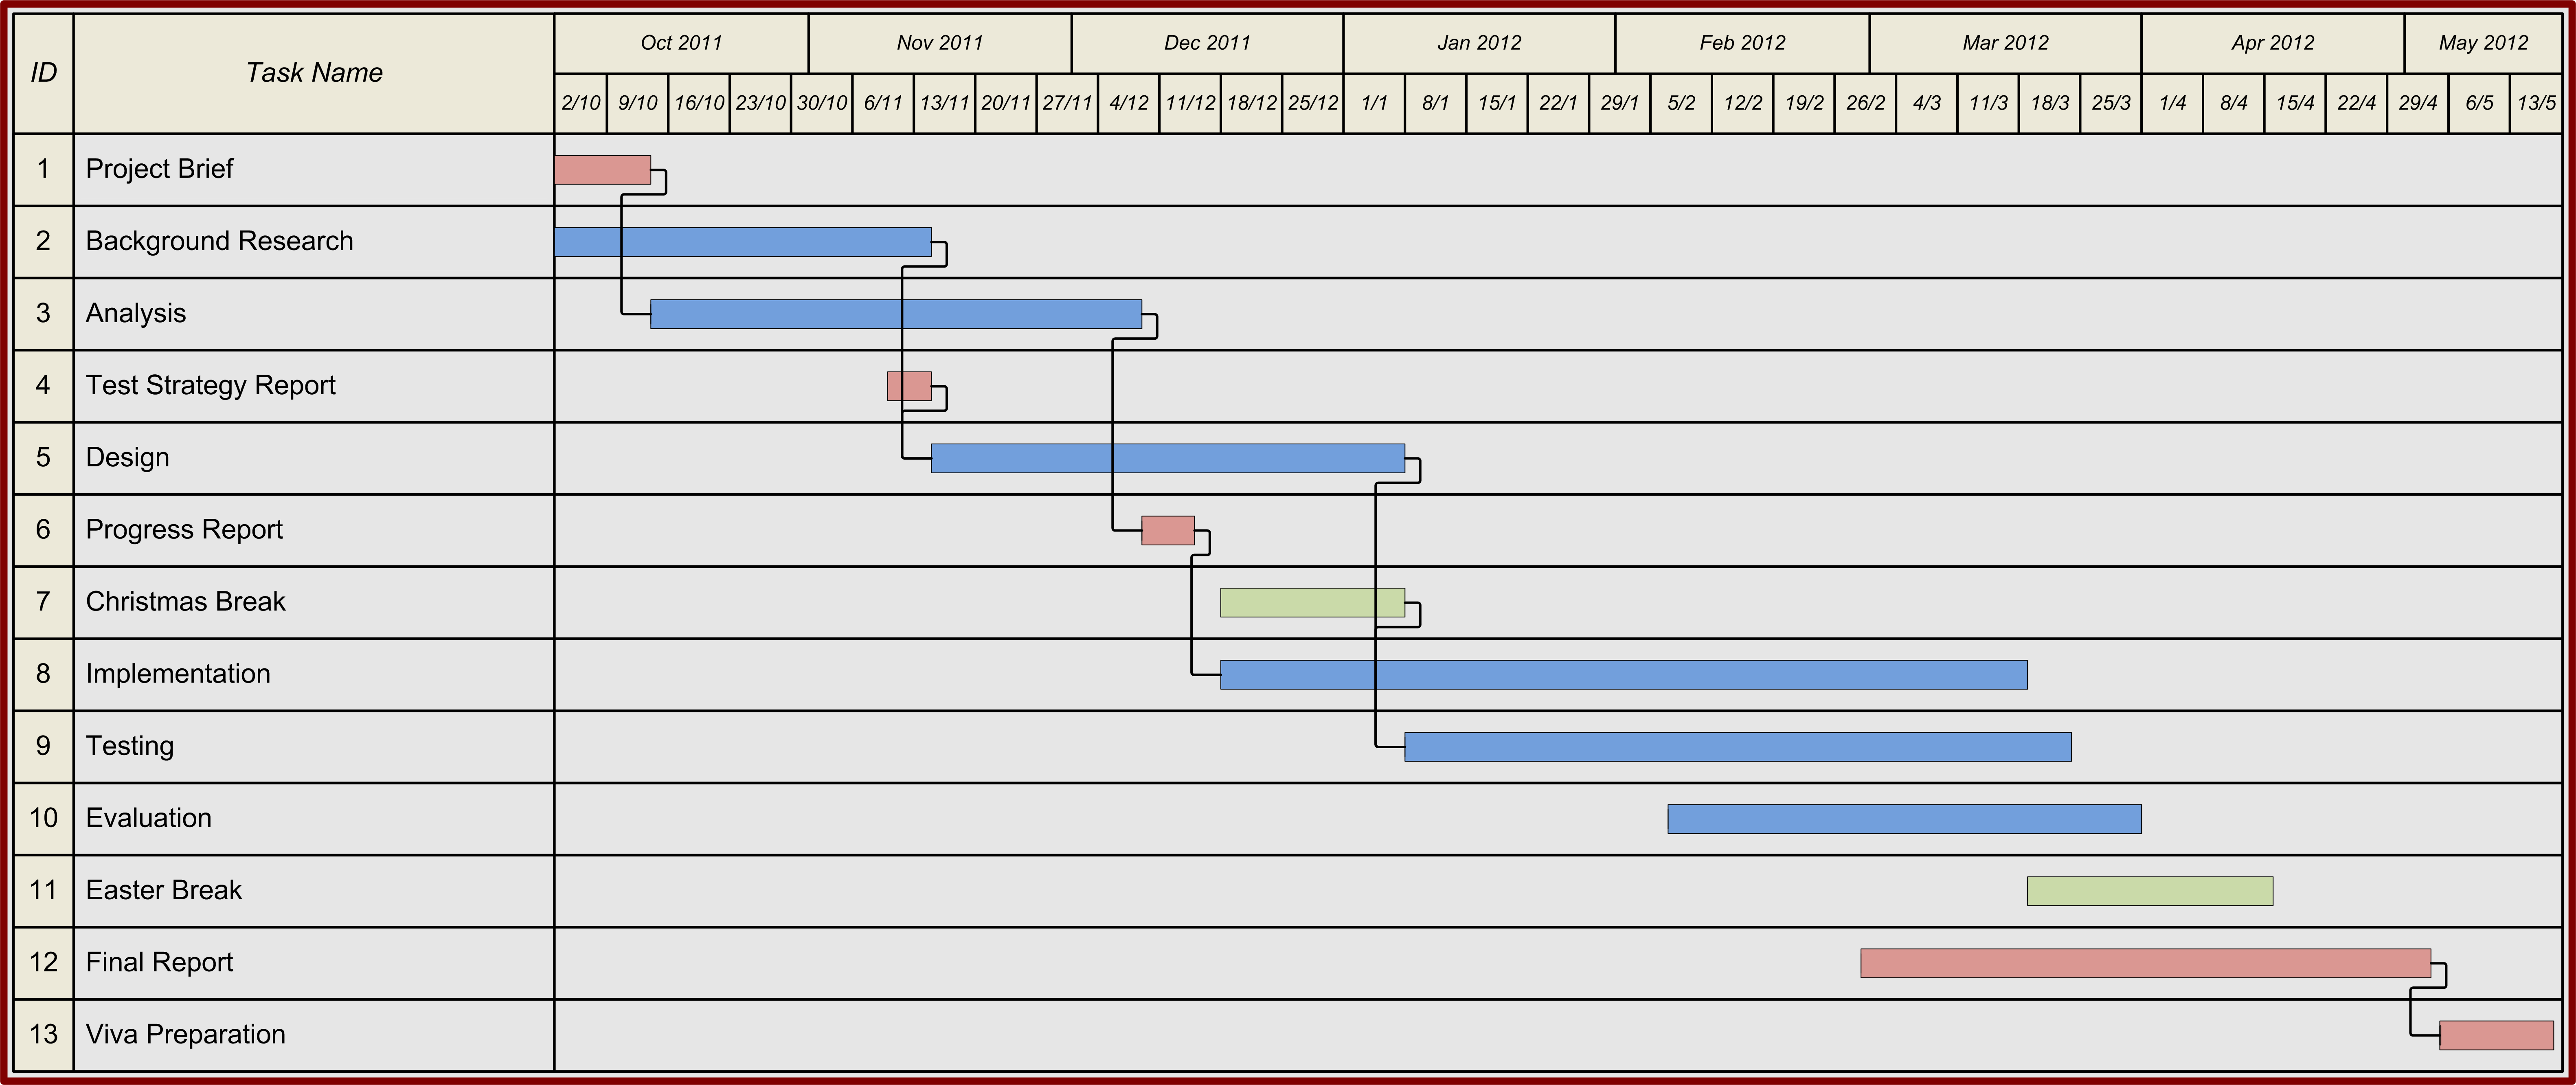
\includegraphics[scale=0.75]{img/3yp-gantt.png}
\caption{Initial Gantt Chart}
\label{fig:chart-1}
\end{figure}
\end{landscape}
\clearpage
\begin{landscape}
\begin{figure}[htb]
\centering
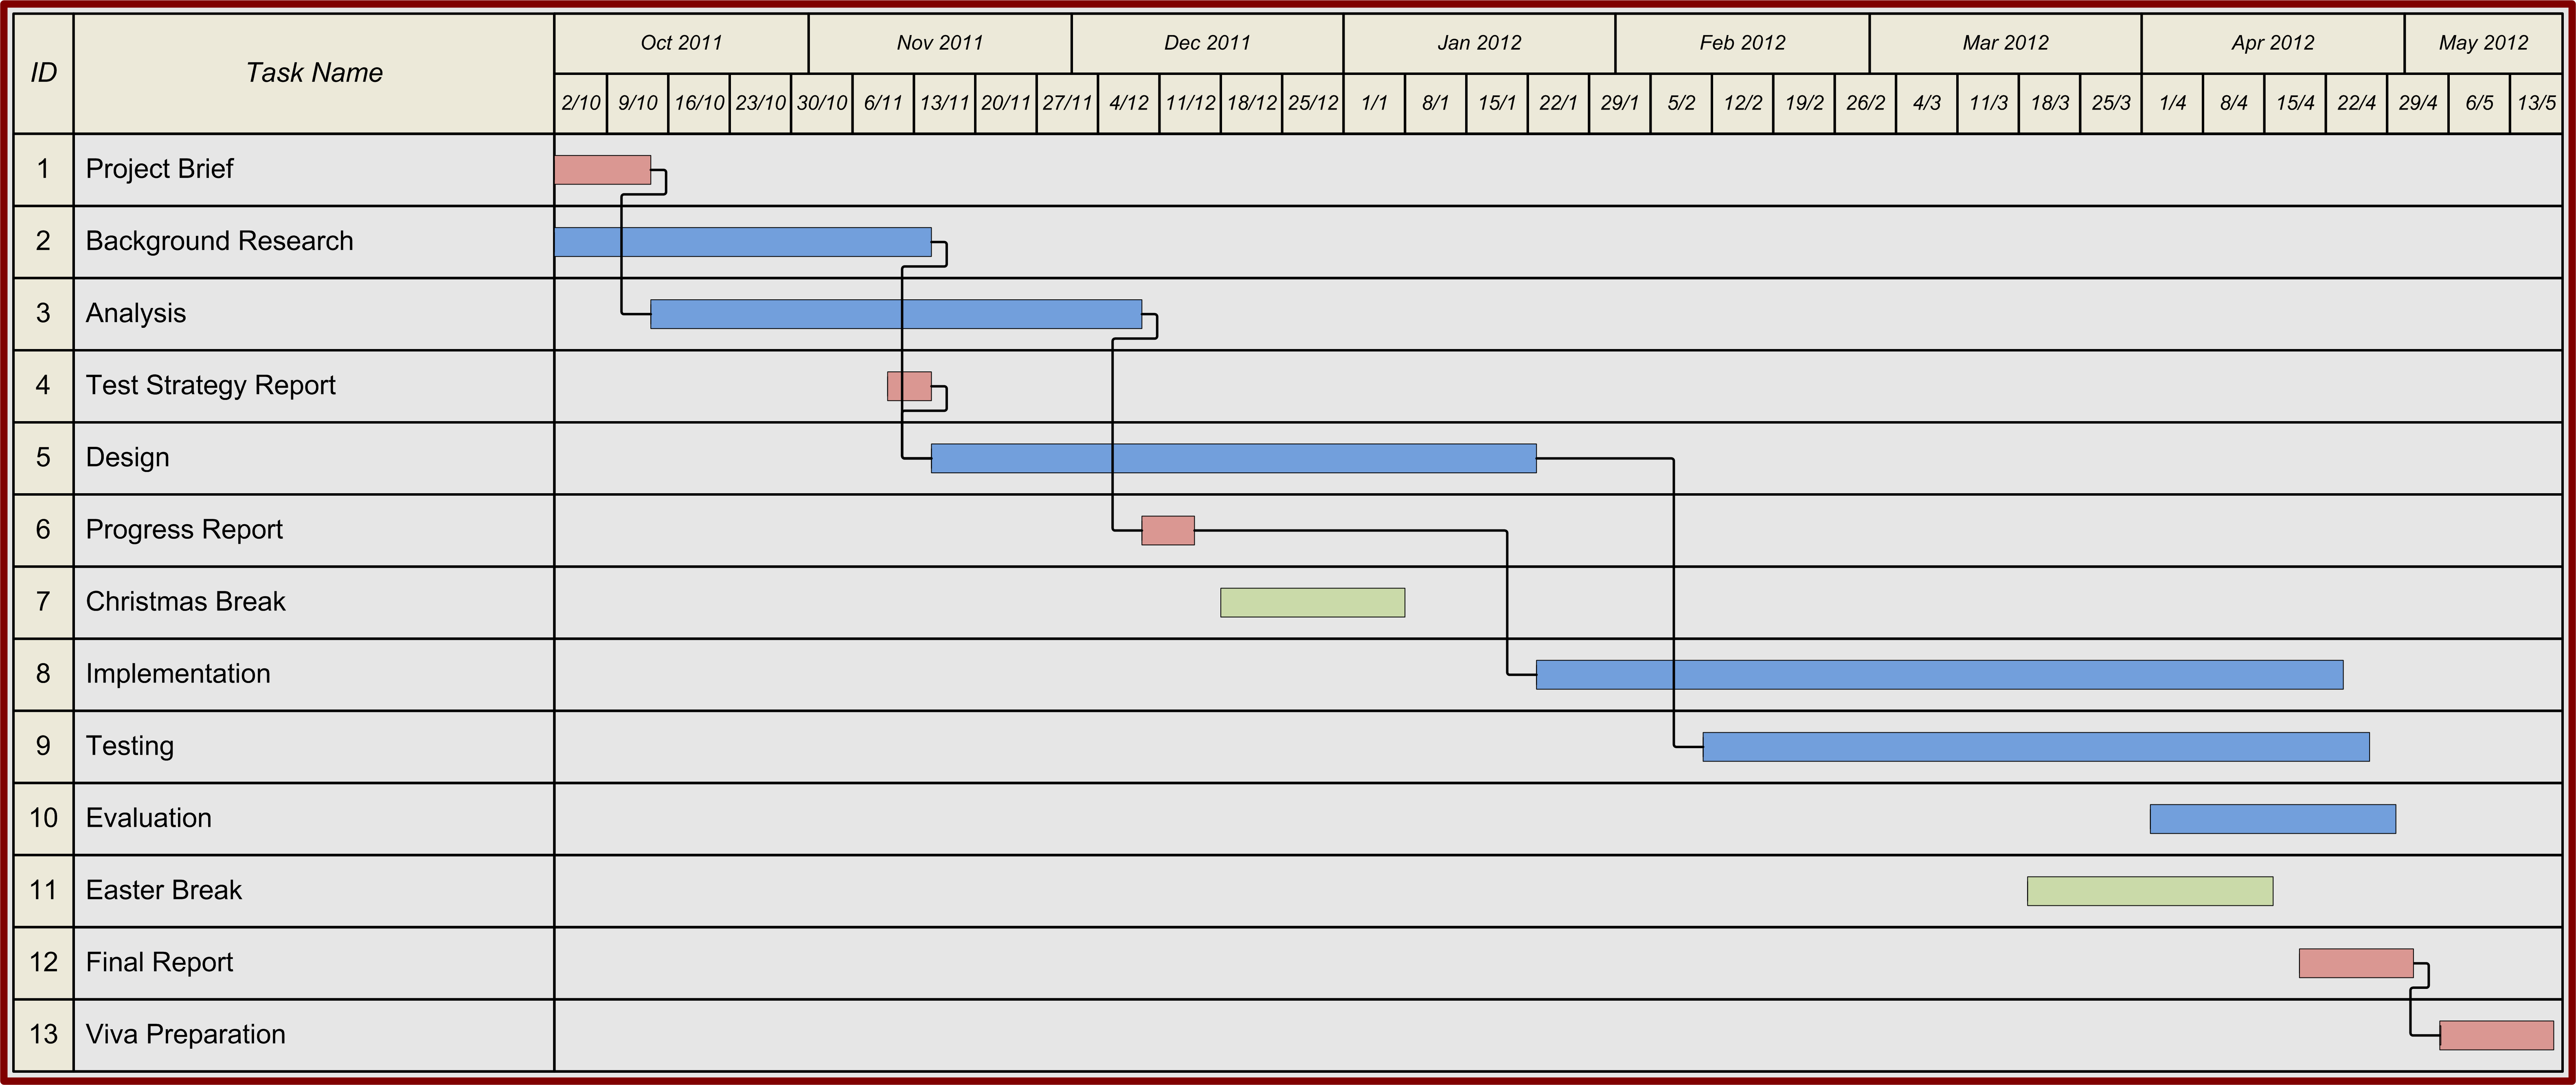
\includegraphics[scale=0.75]{img/3yp-gantt-final.png}
\caption{Final Gantt Chart}
\label{fig:chart-2}
\end{figure}
\end{landscape}


%Conclusions + future work
\section{Conclusion} 
\subsection{URL Classification}

%need to make sure it is clear that we're talking about the URLs rather than the content?
An unknown malicious URL cannot be identified by systems that use signature-based malware detection methods. As a solution, the designed system includes a classifier in order to detect unknown malicious URLs. The classifier relies on pattern matching algorithm used in the Levenshtien distance and has two classes of data; malicious URLs and clean URLs. An unknown URL enterings to the detection system will be classified based on its similarity to the URLs in the dataset. The result of the classification algorithm provides a confidence rate regarding the URL’s maliciousness. Depending on the confidence rate provided, the classifier will then classify whether the given URL should be subject to a heavyweight or lightweight scanning process. However, where the URL is already held within the database, an immediate result is returned confirming with a one hundred percent confidence rate whether or not the URL is malicious. Because a given URL does not need to be checked by multiple scanners simultaneously and unnecessarily, the classifier creates a more efficient and robust detection system. 
 
\subsection{HTML Scanning}

The HTML malware scanner specifically processes trendy keywords from a search engine and within an infected web page to detect a malicious URL. The HTML scanner has been designed based on the repetitive frequency of the trendy keywords within the main URL web page and within the contents of associated hyperlinked web pages. The scanner is efficient and can easily be extended with sophisticated techniques to produce more accurate results. 
 
\subsection{Literature review}
The research in background knowledges gave us better understanding of current 
technologies about malware distribution over the internet. We realised the 
most used approach is to poison search engines which is called Search Engine 
Optimization (SEO), and in order to achieve this the use of trending terms 
is necessary. The processes of a SEO attack was explained, and a method to 
track down SEO campaigns was also introduced. We looked into details about 
how trending keywords can be applied to generate MFA and malicious websites 
such that they can be found by search engines. The significance of search 
engine intervention was proved by Google during Februrary, 2011. \\
Another report acts as our basics of low and high interaction client 
honeypots. It explained passive and active methods for malware detection 
over the web as well as the differences between low and high interaction 
approaches. The automatic malware collecting system they produced inspired 
us the details about how to implement our system. 

\subsection{Wine Explorer and ClamAV scanner}
Wine Explorer provides a lightweight solution for high interaction malware 
detection. It has advantages over virtual machines and emulators including 
short reset time, fast execution and RAM/disk saving, where the potential 
security threat blocks its way to perfection. The program is also approved to 
execute stably, for instance the correctness of the Wine prefix package is 
guaranteed via hash check which avoids external modifications of it. We 
explained the lacking of complete detection as well, which could be 
implemented if we have more time in this project. 
\paragraph{}
We also provide a signiture-based malware scanning powered by ClamAV. The 
HTML crawler in the same program gives links for ClamAV to scan and an 
overall list of malicious links in a webpage can be produced from the 
application. It has fast scanning and executes concurrently which rises 
the system's throughput to a significant amount where disadvantages exists 
such as unprecise link filtering. An improvement could be a deeper level of 
website crawling, and better link processing which requires further amount 
of time to complete. 


\subsection{Capture-HPC}

Capture-HPC is a high interaction client honeypot, a system designed to actively
search for malware by rendering the content at provided URLs. The system is
capable of returning detailed results, and although slow provides a very
accurate simulation of a user browsing with a poorly secured browser and OS.
Capture-HPC integrates easily into the framework using a mysql database to drive
it, although a fair amount of customisation was needed for Capture-HPC to work
in the ECS VM and network infrastructure with additional issues caused by the
security architecture used. Capture-HPC however remains to be a very useful
malware scanner as part of the framework, with further work possible within the
framework to optimise the URLs passed to Capture-HPC so only the most suspicious
URLs are processed. 

\subsection{Framework}

\section{Future development}

The main weakness of the classier in its current form is its processing speed. With the aid of the machine learning algorithm the speed of the URL classification can be improved. At the moment, the pattern-matching algorithm needs to match a given URL with every single URL in the URL database, which contains both malicious and benign URLs. Malicious and benign URLs can be converted into the form of a vector. These two vectors allow additional machine learning methods such as Support Vector Machine (SVM) or Multi-Layers Perceptron (MLP) to be applied. This reduces the need for matching a given URL to every single URL within the URL database. However, converting the URL to a form of a vector is very challenging in terms of implementation effort because the structure of a URL does not have a repetitive pattern.

The second development for the classifier is to use different classification algorithms and then to compares and contrasts their performance. Three machine learning technique algorithms are suggested for implementation, namely; Naïve Bayes, Support Vector Machine (SVM) and Decision Tree. The implementation of these three algorithms requires two datasets; a training and a testing dataset. A list of URLs can be used as training dataset for the classifier and a separate list of URLs is required for the testing dataset. URLs in the testing dataset should be completely different from those URLs in the training dataset. The important aspect involves the selection of URL features for classification. Many features can be considered such as; length of the URL, number of forward slashes “/”or the number of dots “.” used in the URL structure. Features extracted from the URL’s structure are used as input for the classifier. The classifier will use extracted features to distinguish a malicious URL from the benign URL. 

In the current system the HTML malware scanner uses a URL and a keyword as the input and based on the frequency of the keyword in the web page of the given URL decides whether the URL is malicious or clean. An alternative design for the HTML scanner involves continuously updating a database with a feed of new trendy keywords so that the HTML scanner’s only input requirement is a given URL. The challenging part of this model is designing of a trendy keyword database, with each trendy keyword belonging to a group of keywords that have the same topic. The database will be connected to a list of selected trusted website such as BBC News. In turn, the database can be updated with any new trendy keywords being used on the News website, with old keywords being removed from the database after a predefined time period e.g. one month. In this model, the scanner decision is not only based on one trendy-keyword, it is based on a group of keywords connected to the trendy keyword topic within the database. Therefore, ensuring a more reliable result is provided by the malware scanner.

Another option for the design of the HTML malware scanner involves considering the features of the web page related to each URL. In this method, a list of features of the webpage is extracted. This method is very similar to the one already suggested for the classifier. Again, there is a list of training dataset and testing dataset for the classifier, but instead the extracted features from web page will used as an input for the classifier. The web page features may be the number of hyperlinks in the webpage, number of lines, word count and functions (JavaScript keywords).

After training the classifier, some features may provide more useful results such as the use of JavaScript function in the web page. Hence, the features that produce the most accurate results will be selected for classification. Although the latter model does not consider the relationship between the trendy keyword term and the malicious URLs, a powerful system with an updated database and classifier can be created by combining the above two models. As a result of which, the database would contain a list of trendy keyword terms updated from trusted websites and the classifier would be capable of identifying unknown malicious URLs relating to the trendy keyword term.

The malware detection system that employs machine-learning techniques has a few advantages. The system can overcome the problem of detecting an unknown malware and also polymorphic malwares. In addition, it is very efficient and resilient in comparison with other malware detection techniques. Moreover, the adapted techniques in this system make it difficult for malware writers to bypass the detection system. 









%references
\addcontentsline{toc}{section}{References}
\bibliographystyle{IEEEtran}
\bibliography{final-report,rfc,i-d,tag1g09,cso1g09,nv2g09,wl15g09}{}

%Appendices
\appendix
\section{Project Brief}
%DNS\nomenclature{DNS}{Domain Name Service}

\newpage
\mbox{}
\newpage
\mbox{}
\newpage

\section{List of Abbreviations}
\renewcommand{\nomname}{}
\printnomenclature

\clearpage
\section{User Manual}
\label{sec:manual}


\clearpage
\section{Contents of Source Disk}

Each directory has a README files describing its contents.

\subsection{Directories}
\begin{enumerate}
\item\texttt{db-tools/} - Node database tools and Icinga Templates
\begin{enumerate}
 \item\texttt{bottle.py} - copy of Bottle.py web framework.
 \item\texttt{list-serve.py} - normal python version of list-serve using default sever.
 \item\texttt{list-serve.wsgi} - wsgi compatible version of the server.
 \item\texttt{templates/} - templates used for Icinga config generation.
 \item\texttt{update-icinga.py} - script for taking values from the node database, and creating
Icinga configuration files.
 \item\texttt{upload-db.py} - script for adding new nodes to the database.
\end{enumerate}
\item\texttt{edumond-node/} - Configuration running on the wireless node
\begin{enumerate}
 \item\texttt{lighttpd/} - copy of /etc/lighttpd, containing lighttpd.conf with fastcgi
 \item\texttt{lua/} - copy of /usr/lib/lua, containing json.lua and rad-check.lua
 \item\texttt{rad-check/} - copy of /etc/rad-check, containing config.lua and client and server keys/certs
 \item\texttt{magnet} - binary used by fastcgi to run Lua scripts with POST data.
 \item\texttt{packages} - list of openwrt packages installed
 \item\texttt{send\_nsca.cfg} - copy of /etc/send\_nsca.conf, configured to
contact Icinga server
\end{enumerate}
\item\texttt{kanga-config/} - Configuration for Icinga, FreeRADIUS, and PNP4Nagios
\begin{enumerate}
 \item\texttt{www/} - copy of /var/www, node serving code in www/wsgi
 \item\texttt{httpd/} - copy of /etc/httpd, nodes server set up in httpd/conf/httpd.conf
 \item\texttt{raddb/} - copy of /etc/raddb, FreeRadius configuration files.
 \item\texttt{nagios/} - copy of /etc/nagios, contains NSCA configuration in nagios/nsca.cfg
 \item\texttt{icinga/} - copy of /etc/icinga, Icinga configuration files
\begin{enumerate}
                \item icinga/objects/matrix-hosts - test device defenitions
                \item icinga/objects/matrix.cfg - general test configuration
                \item icinga/objects/commands.cfg - contains added commands
                \item icinga/objects/templates.cfg - contains service templates
\end{enumerate}
 \item\texttt{nodedb.sql} - Dump of the MySQL database of the nodes
\end{enumerate}
\item\texttt{kangab-config/} - Configuration for second FreeRADIUS server.
\begin{enumerate}
 \item\texttt{raddb/} - copy of /etc/raddb, FreeRadius configuration files.
\begin{enumerate}
                \item raddb/clients.conf - clients with secrets
                \item raddb/proxy.conf - realm configuration
\end{enumerate}
\end{enumerate}
\item\texttt{rad-check/} - Test data generation code
\begin{enumerate}
 \item\texttt{credcheck.lua} - fastcgi response script
 \item\texttt{eapol\_test} - cross-compiled eapol\_test tool
 \item\texttt{edumond.lua} - Lua credential exchange and testing script
 \item\texttt{edumond.py} - deprecated python version
 \item\texttt{index.lua} - debug script
 \item\texttt{json-LICENCE.txt} - License for Lua JSON library
 \item\texttt{json.lua} - JSON library
 \item\texttt{magnet.c} - modified magnet.c source code to pass POST data.
 \item\texttt{rad-check.lua} - Lua script for automating eapol\_test
 \item\texttt{rad-check.py} - deprecated python version
 \item\texttt{templates/} - wpa\_supplicant type templates for eapol\_test
\end{enumerate}
\item\texttt{security/} - PKI and certificates
\begin{enumerate}
 \item\texttt{CA/} - copy of /etc/pki/CA, containing CA certificate and private key,
                with a registry of certificate requests and issues 
 \item\texttt{secure/} - copy of /root/secure, x509 certificates and keys used during
                the testing of the system. Because the test system is still
                live, passphrases for keys are not provided.
\end{enumerate}
\end{enumerate}

\clearpage
\section{Report Allocation}
\label{sec:words}
\begin{center}
%\begin{table}
\begin{tabularx}{\linewidth}{|XXX|}
\hline
Group Member & report section\\ \hline
Thomas Grainger & Malware Lists\\
& Specification\\
& Customer Interaction\\
& Architectural Design\\
& Trend Analysis Design\\
& URL Descovery Design\\ \hline

Weike Liao & Literature Review \\
& Architectural Design \\
& Trend Analysis Implemenation \\
& URL Descovery Implemenation \\
& Wine \\
& ClamAV \\ \hline

Chris Orchard & Description \\
& Capture HPC \\
& Group Approach \\ \hline

Nafiseh Vahabi & Literature Review  \\
& Related Work \\
& Manual HTML \\
& Classifier \\
& Future Development \\ \hline
\hline
\end{tabularx}
%\end{table}
\end{center}

%TODO: following sections:
%       project description
%       literature review
%       design + spec.
%       justification of approact
%       project control: past, future
%       gantt chart


\end{document}
